% FAS2GraphTheoryTikZ-002.tex
% Asset ID: FAS2GraphTheoryTikZ-002
% Unit: FAS2 Further AS 2 Applied Mathematics
% Topic Code: FAS2-GRAPH
% Topic Name: Graph theory
% Topic ID: FAS2GraphTheory
% Related lesson file: FAS2_graph_theory_lesson.md
% Source: CCEA FAS2-GRAPH traversability boundary plus uploaded lesson PDF and transcript on Euler's handshaking lemma
% Purpose: Show how the number of odd vertices controls possible Eulerian traversability.

\documentclass[tikz,border=8pt]{standalone}
\usepackage{tikz}
\usetikzlibrary{calc,positioning}
\definecolor{Canvas}{HTML}{FAF9F6}
\definecolor{Ivory}{HTML}{FFFFF0}
\definecolor{Line}{HTML}{2C2C2E}
\definecolor{Divider}{HTML}{E5E5EA}
\definecolor{Gold}{HTML}{C5A059}
\definecolor{SoftGold}{HTML}{D4AF37}
\definecolor{Blush}{HTML}{FBEFEF}

\begin{document}
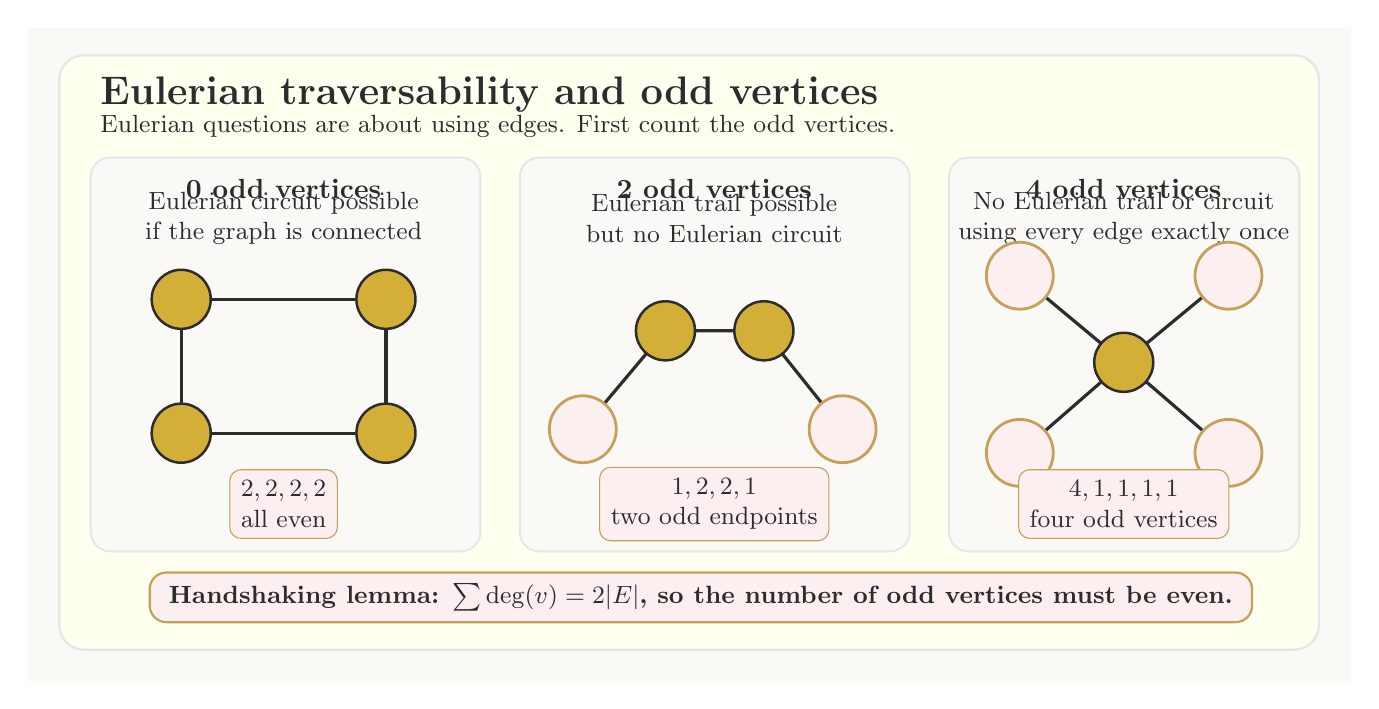
\begin{tikzpicture}[
  vertex/.style={circle,draw=Line,fill=SoftGold,line width=0.9pt,minimum size=7.5mm,inner sep=0pt},
  oddvertex/.style={circle,draw=Gold,fill=Blush,line width=1pt,minimum size=8.5mm,inner sep=0pt},
  edge/.style={draw=Line,line width=1.15pt,line cap=round},
  panel/.style={draw=Divider,fill=Canvas,rounded corners=7pt,line width=0.7pt},
  labeltext/.style={font=\small,text=Line,align=center},
  heading/.style={font=\bfseries,text=Line,align=center},
  formula/.style={fill=Blush,draw=Gold,rounded corners=4pt,inner sep=4pt,font=\small,text=Line,align=center}
]
\fill[Canvas] (-1.0,-1.1) rectangle (15.8,7.2);
\draw[draw=Divider,fill=Ivory,rounded corners=9pt,line width=0.8pt] (-0.6,-0.7) rectangle (15.4,6.85);
\node[anchor=west,font=\Large\bfseries,text=Line] at (-0.2,6.35) {Eulerian traversability and odd vertices};
\node[anchor=west,font=\small,text=Line] at (-0.2,5.95) {Eulerian questions are about using edges. First count the odd vertices.};
\draw[panel] (-0.2,0.55) rectangle (4.75,5.55);
\draw[panel] (5.25,0.55) rectangle (10.2,5.55);
\draw[panel] (10.7,0.55) rectangle (15.15,5.55);
\node[heading] at (2.25,5.15) {0 odd vertices};
\node[labeltext] at (2.25,4.78) {Eulerian circuit possible\\if the graph is connected};
\coordinate (A1) at (0.95,3.75); \coordinate (B1) at (3.55,3.75); \coordinate (C1) at (3.55,2.05); \coordinate (D1) at (0.95,2.05);
\draw[edge] (A1)--(B1)--(C1)--(D1)--(A1);
\node[vertex] at (A1) {}; \node[vertex] at (B1) {}; \node[vertex] at (C1) {}; \node[vertex] at (D1) {};
\node[formula] at (2.25,1.15) {$2,2,2,2$\\all even};
\node[heading] at (7.72,5.15) {2 odd vertices};
\node[labeltext] at (7.72,4.78) {Eulerian trail possible\\but no Eulerian circuit};
\coordinate (A2) at (6.05,2.1); \coordinate (B2) at (7.1,3.35); \coordinate (C2) at (8.35,3.35); \coordinate (D2) at (9.35,2.1);
\draw[edge] (A2)--(B2)--(C2)--(D2);
\node[oddvertex] at (A2) {}; \node[vertex] at (B2) {}; \node[vertex] at (C2) {}; \node[oddvertex] at (D2) {};
\node[formula] at (7.72,1.15) {$1,2,2,1$\\two odd endpoints};
\node[heading] at (12.92,5.15) {4 odd vertices};
\node[labeltext] at (12.92,4.78) {No Eulerian trail or circuit\\using every edge exactly once};
\coordinate (O3) at (12.92,2.95); \coordinate (A3) at (11.6,4.05); \coordinate (B3) at (14.25,4.05); \coordinate (C3) at (11.6,1.8); \coordinate (D3) at (14.25,1.8);
\draw[edge] (O3)--(A3); \draw[edge] (O3)--(B3); \draw[edge] (O3)--(C3); \draw[edge] (O3)--(D3);
\node[vertex] at (O3) {}; \node[oddvertex] at (A3) {}; \node[oddvertex] at (B3) {}; \node[oddvertex] at (C3) {}; \node[oddvertex] at (D3) {};
\node[formula] at (12.92,1.15) {$4,1,1,1,1$\\four odd vertices};
\draw[draw=Gold,fill=Blush,rounded corners=6pt,line width=0.8pt] (0.55,-0.35) rectangle (14.55,0.28);
\node[font=\small\bfseries,text=Line] at (7.55,-0.03) {Handshaking lemma: $\sum \deg(v)=2|E|$, so the number of odd vertices must be even.};
\end{tikzpicture}
\end{document}
